\section{Theoretische Grundlagen}
\label{sec:theoretGrundl}
Dieses Kapitel behandelt die theoretischen Grundlagen für verwendete Verfahren, Hardware und Software. Es hat die Aufgabe den Leser:innen für das Verständnis essentielle Informationen zu übermitteln.
\subsection{Globales Positionsbestimmungssystem}
\label{subsec:tGPS}
Das \ac{GPS} ist ein gängiges Navigationssystem, um die geografische Position zu ermitteln. Ursprünglich wurde \ac{GPS} für militärische Zwecke entwickelt und wird heutzutage vom Verteidigungsministerium der USA betrieben.\\
\ac{GPS} ist satellitengestützt und umfasst eine Anzahl von 32 Satelliten in der Erdumlaufbahn, wovon mindestens vier eine Verbindung mit dem GPS-Empfängermodul haben müssen, um die Position bestimmen zu können. Drei dieser Satelliten sind für die Erfassung der Längen- und Breitengrade sowie die der Höhe notwendig, die Verbindung mit einem vierten Satelliten ermöglicht die Synchronisation der Uhr des Empfängers, mit der der Satelliten. Dies ist besonders ausschlaggebend, da nur bei einer exakten Übereinstimmung der Zeiten, die Position korrekt berechnet werden kann. Um die Position zu berechnen, wird die Zeit gemessen, die das Signal vom Satelliten zum Empfänger benötigt und in eine Distanz umgerechnet. Mithilfe der Entfernungen zu mehreren Satelliten vom Empfänger, kann über Triangulation die geografische Lage auf der Erdoberfläche ermittelt werden.\\
Die Genauigkeit der Positionserfassung variiert zwischen 13 Meter und 1 Millimeter. Abweichungen unter einem Meter sind allerdings fast nur mit professioneller, beziehungsweise militärischer Ausrüstung erreichbar. Mit Komponenten aus den Hobby-Elektronikbereich sowie in Smartphones, sind Genauigkeiten zwischen 13 und 3 Metern realistisch möglich.\\
Die Daten werden standardisiert im \ac{NMEA}-Format über eine serielle Schnittstelle ausgegeben. (\cite{schnabelGPS})


\subsection{Inertiale Messeinheit}
\label{subsec:tIMU}
Eine \ac{IMU} z. Dt. inertiale Messeinheit kombiniert mehrere verschiedene Sensoren zur Bestimmung von Lage, Beschleunigungen und Position im dreidimensionalen Raum. Um eine zuverlässige Ermittlung dieser Werte zu gewährleisten, werden Beschleunigungsmessung, Rotationsgeschwindigkeitsmessung (und in einigen Fällen auch die Messung des Magnetfeldes der Erde) kombiniert. Inertiale Messeinheiten werden unter anderem für die Navigation von Flugzeugen, Raumschiffen und Schiffen verwendet. In der Automobilindustrie werden \ac{IMU}s verwendet, um das Fahrverhalten von Autos zu bestimmen und dieses zu verbessern.\\
Die \ac{IMU} liefert die Beschleunigungen sowohl in x-, y- als auch z-Richtung, die Winkelgeschwindigkeiten um die x-, y- als auch z-Achse (und in manchen Fällen die magnetische Feldstärke in x-, y- als auch z-Richtung). Um die Lage zu bestimmen können die Beschleunigungssensoren verwendet werden, indem die Lage der Erdbeschleunigung im dreidimensionalen Raum ermittelt wird, dies funktioniert allerdings nur, solange der Sensor sich in Ruhelage befindet. Alternativ können die Rotationsgeschwindigkeiten integriert werden, dies ergibt aber aufgrund von Messfehlern nach einiger Zeit Abweichungen (drift).\\ Um eine fehlerfreie Ermittlung der Lage zu ermöglichen kann Sensorfusion betrieben werden. Darunter versteht man einen Prozess, der Signale von zwei oder mehr Sensoren zusammenfasst. Im Falle einer \ac{IMU} kann die Ermittlung mittels Accelerometern, Gyroskopen und Magnetometern wie in Sektion \ref{subsec:IMUprogram} beschrieben kombiniert werden.
(\cite{UCAM-CL-TR-696})
\begin{figure}[h]
\centering
\tdplotsetmaincoords{60}{120}
\tdplotsetrotatedcoords{-15}{20}{25}
\begin{tikzpicture}
		[tdplot_rotated_coords,
			cubefront/.style={very thick,black},
			cubeback/.style={thick,dashed,black},
			grid/.style={very thin,gray},
			axis/.style={->,red,thick},
			rotated axis/.style={->,darkgreen,thick}]

	\foreach \x in {-0.25,0,...,2.25}
		\foreach \y in {-0.25,0,...,2.25}
		{
			\draw[grid] (\x,-0.25) -- (\x,2.25);
			\draw[grid] (-0.25,\y) -- (2.25,\y);
		}
			
	\draw[axis,tdplot_main_coords] (0,0,0) -- (3,0,0) node[anchor=west]{$x$};
	\draw[axis,tdplot_main_coords] (0,0,0) -- (0,3,0) node[anchor=north west]{$y$};
	\draw[axis,tdplot_main_coords] (0,0,0) -- (0,0,3) node[anchor=west]{$z$};


	\draw[rotated axis] (0,0,0) -- (3,0,0) node[anchor=west]{$x'$};
	\draw[rotated axis] (0,0,0) -- (0,3,0) node[anchor=south west]{$y'$};
	\draw[rotated axis] (0,0,0) -- (0,0,3) node[anchor=west]{$z'$};

	\draw[cubeback] (0,0,0) -- (0,2,0);
	\draw[cubefront] (0,2,0) -- (2,2,0);
	\draw[cubefront] (2,2,0) -- (2,0,0);
	\draw[cubeback] (2,0,0) -- (0,0,0);
	
	\draw[cubefront] (0,0,1) -- (0,2,1);
	\draw[cubefront] (0,2,1) -- (2,2,1);
	\draw[cubefront] (2,2,1) -- (2,0,1);
	\draw[cubefront] (2,0,1) -- (0,0,1);
	
	\draw[cubeback] (0,0,0) -- (0,0,1);
	\draw[cubefront] (0,2,0) -- (0,2,1);
	\draw[cubefront] (2,0,0) -- (2,0,1);
	\draw[cubefront] (2,2,0) -- (2,2,1);
	
\end{tikzpicture}
\caption{Eine \ac{IMU} in einem \ac{3D}-Koordinatensystem}
\label{fig:IMU3D}
\end{figure}

\subsection{Hall-Effekt-Sensor}
\label{subsec:tHall}
Wenn ein elektrischer Leiter mit Strom durchflossen wird, so bewegen sich die Elektronen geradlinig in eine Richtung. Es sei denn der Leiter befindet sich im Wirkungsbereich eines Magnetfeldes (z.B. eines Permanentmagneten), wobei die Feldlinien normal zur Elektronenbahn stehen. Die Elektronen werden dann auf eine gekrümmte Bahn abgelenkt, da das Magnetfeld des Leiters, dem des Permanentmagneten entgegenwirkt. Deswegen befinden sich auf der Seite des Leiters mit der Bahn-Krümmung mehr Elektronen, was einen Potentialunterschied zur Folge hat. Dieser variiert je nach Position des Permanentmagneten. Sogenannte Hall-Effekt-Sensoren funktionieren auf diesem Prinzip, sind allerdings aus einem Halbleitermaterial aufgebaut. Man kann hierbei zwischen analogen und digitalen Hall-Senoren unterscheiden.\\
Wie der Name vermuten lässt, ist das Ausgangssignal eines analogen Hall-Sensors linear variabel und direkt proportional zur magnetischen Flussdichte. Die Grenzen der Ausgangsspannung werden von der Versorgungsspannung definiert. Auf digitalen Hall-Sensoren befindet sich ein bistabiler Stromkreis, ein sogenannter Schmitt-Trigger, welcher den Ausgang auf logisch 0 oder 1 setzt, je nachdem, ob der bestimmte Grenzwert überschritten wird, oder nicht. (\cite{rsHALL})

\subsection{Infrarot-Lichtschranke}
\label{subsec:tIR}
Lichtschranken gehören zur sogenannten Optoelektronik und geben ein Signal aus, wenn ein Lichtstrahl unterbrochen wird. Ein Lichtschranke besteht aus einem Sender und einem Empfänger. Der Sender besteht grundsätzlich aus einer Leuchtdiode, wobei hier zwischen sichtbarem und unsichtbarem Licht unterschieden wird. Als, für das menschliche Auge, unsichtbare Lichtquelle werden meist \ac{IR}-Leuchtdioden eingesetzt, welche eine Wellenlänge von 880-940 Nanometer aufweisen. Der Empfänger einer Lichtschranke besteht grundsätzlich aus einer Photodiode, wessen Signal zusätzlich verstärkt wird. Außerdem wird zwischen verschiedenen Konfigurationen des Senders und Empfängers unterschieden, wobei hier auf die sogenannte Einwegkonfiguration eingegangen wird. Der Sender und der Empfänger stehen sich dabei direkt gegenüber. In Form einer \ac{IR}-Gabellichtschranke im Hobbyelektronik-Bereich befinden sich diese auf einer gemeinsamen Platine (siehe Abbildung \ref{fig:IR}) und bei einer Unterbrechung des Lichtstrahls wird der Ausgang auf logisch 1, beziehungsweise, in diesem Fall, +3.3 Volt gesetzt.
(\cite{huschke2000lichtschranken})
\begin{figure}[h]
\centering
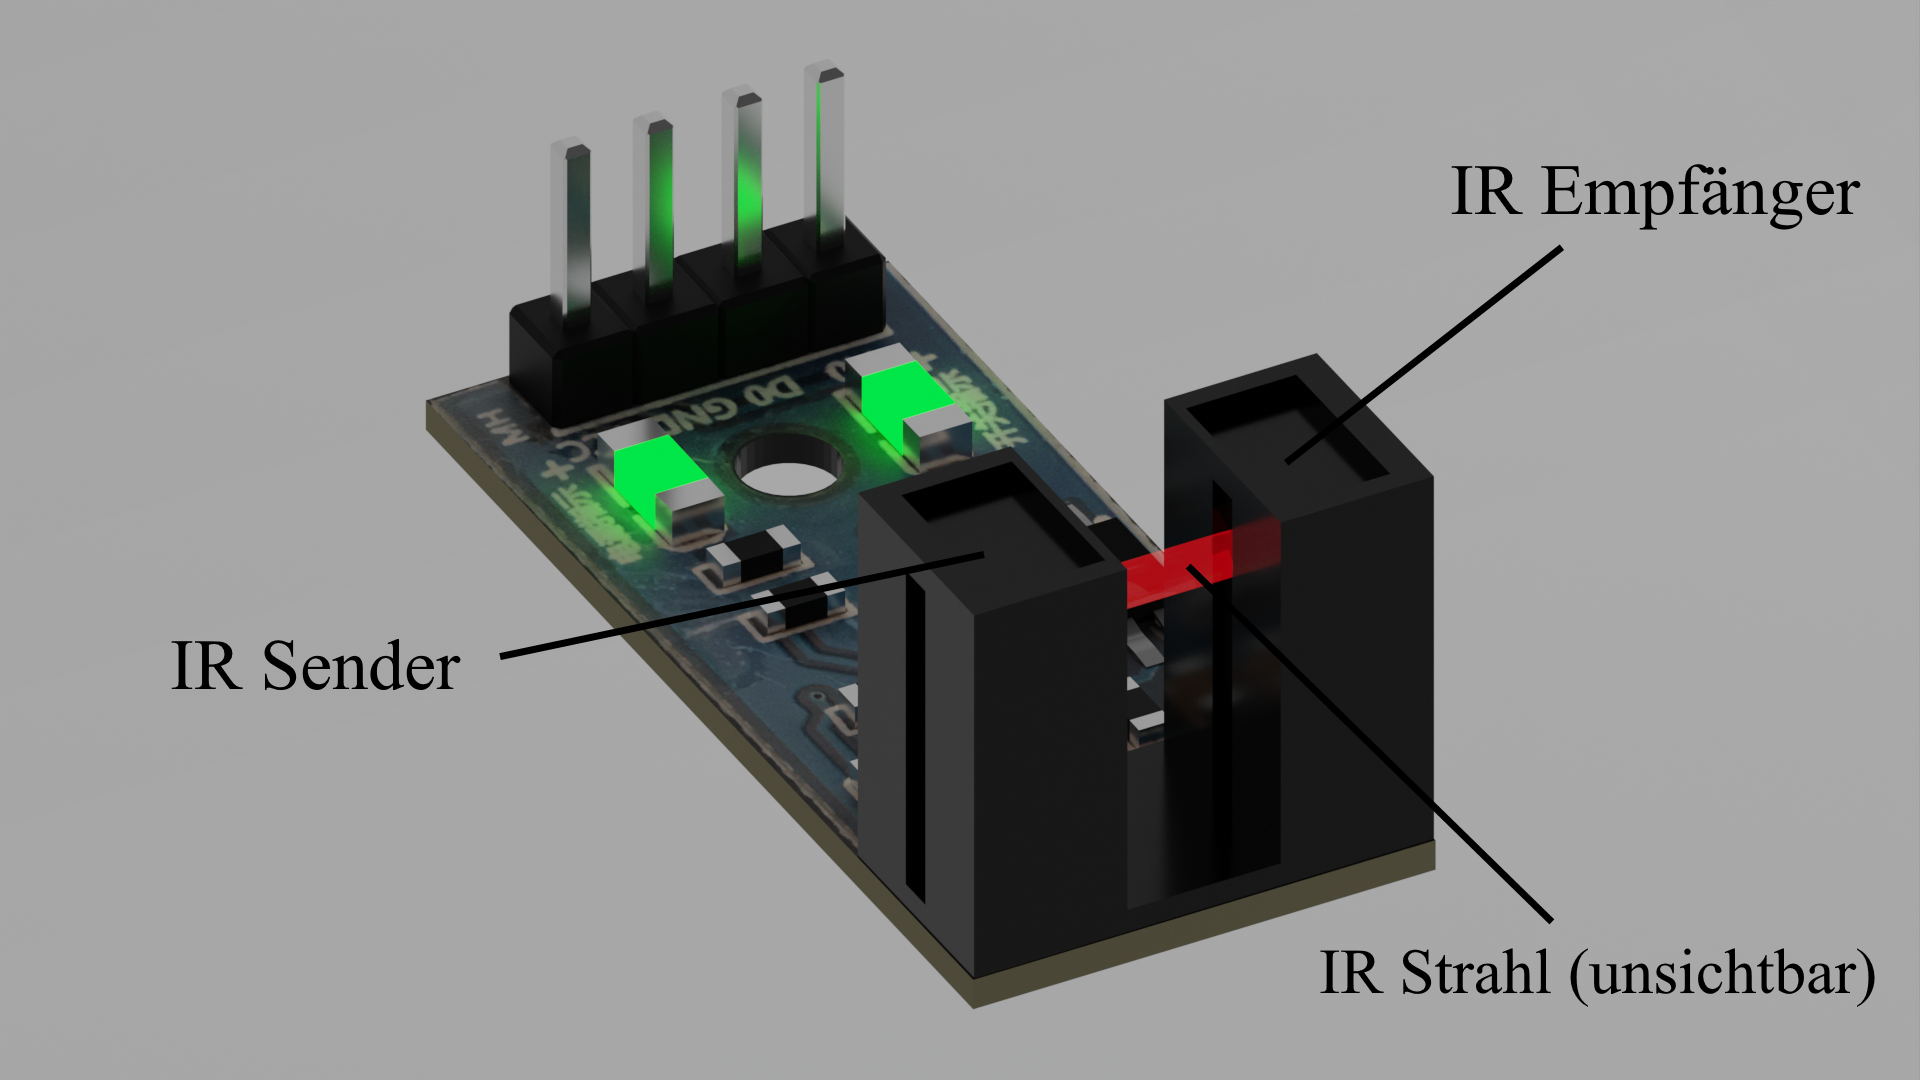
\includegraphics[scale=0.2]{IR.png}
\caption{IR-Gabellichtschranke}
\label{fig:IR}
\end{figure}

\subsection{Drehzahlregler}
\label{subsec:tESC}
Wie in Sektion \ref{sec:Auto} erklärt wird, dient ein bürstenloser Gleichstrommotor als Antrieb des Modellautos. Um die Drehzahl dieses Motors regeln zu können ist ein sogenannter \ac{ESC}, z. Dt. Drehzahlregler, notwendig. Anders als bei Bürstenmotoren wird ein Drehfeld mit mehreren Spulen von insgesamt drei Phasen, im Stator erzeugt. Am Rotor (Motorwelle) sind Permanentmagnete dementsprechend angebracht, diese werden von den Magnetfeldern der Spulen sequentiell angezogen, wodurch sich die Welle zu drehen beginnt. Das Erzeugen dieses Drehfeldes, also das zeitversetzte Ein- und Ausschalten der Phasen, übernimmt der \ac{ESC}. Das Signal jeder Phase ist prinzipiell ein Rechtecksignal. Über die Ein- und Ausschaltzeit werden die Spulen einer Phase im richtigen Moment aktiviert und deaktiviert. Alle drei Signale werden zeitlich so versetzt, dass ein rotierendes Magnetfeld entsteht. Die Frequenz dieser Signale gibt schließlich die Drehzahl vor. Die Information der Drehzahl erlangt der \ac{ESC} über den Empfänger des Funksystems.
(\cite{ESC})

\subsection{Raspberry Pi Zero 2 W}
\label{subsec:tRasPi}
Der Raspberry Pi Zero 2 W ist ein Einplatinencomputer von Raspberry Pi. Mit einem 1 \ac{GHz} quad-core 64-bit Arm Prozessor, 512 \ac{MB} \ac{SDRAM}, eingebauten \ac{WLAN}- und Bluetooth-Modulen und 40 Pins für \ac{GPIO}, \ac{SPI}, \ac{I2C}, \ac{UART} und Spannungsversorgung stellt er ein umfangreiches Paket für die Interaktion mit diverser Sensorik dar. Wie bereits erwähnt, handelt es sich bei dem Raspberry Pi Zero 2 W um einen Einplatinencomputer. Das bedeutet, dass dieser alle Funktionen eines konventionellen Computers auf einer Platine bereit stellt. Mithilfe des Micro-\ac{USB} Anschlusses kann der Raspberry Pi mit externer Peripherie und externen Speichermedien kommunizieren, mithilfe des Mini \ac{HDMI} Ports kann ein externes Display verbunden werden. Die Spannungsversorgung des Raspberry Pi erfolgt über einen zweiten Micro-\ac{USB} Anschluss.
(\cite{Raspi})
\begin{figure}[h]
\centering
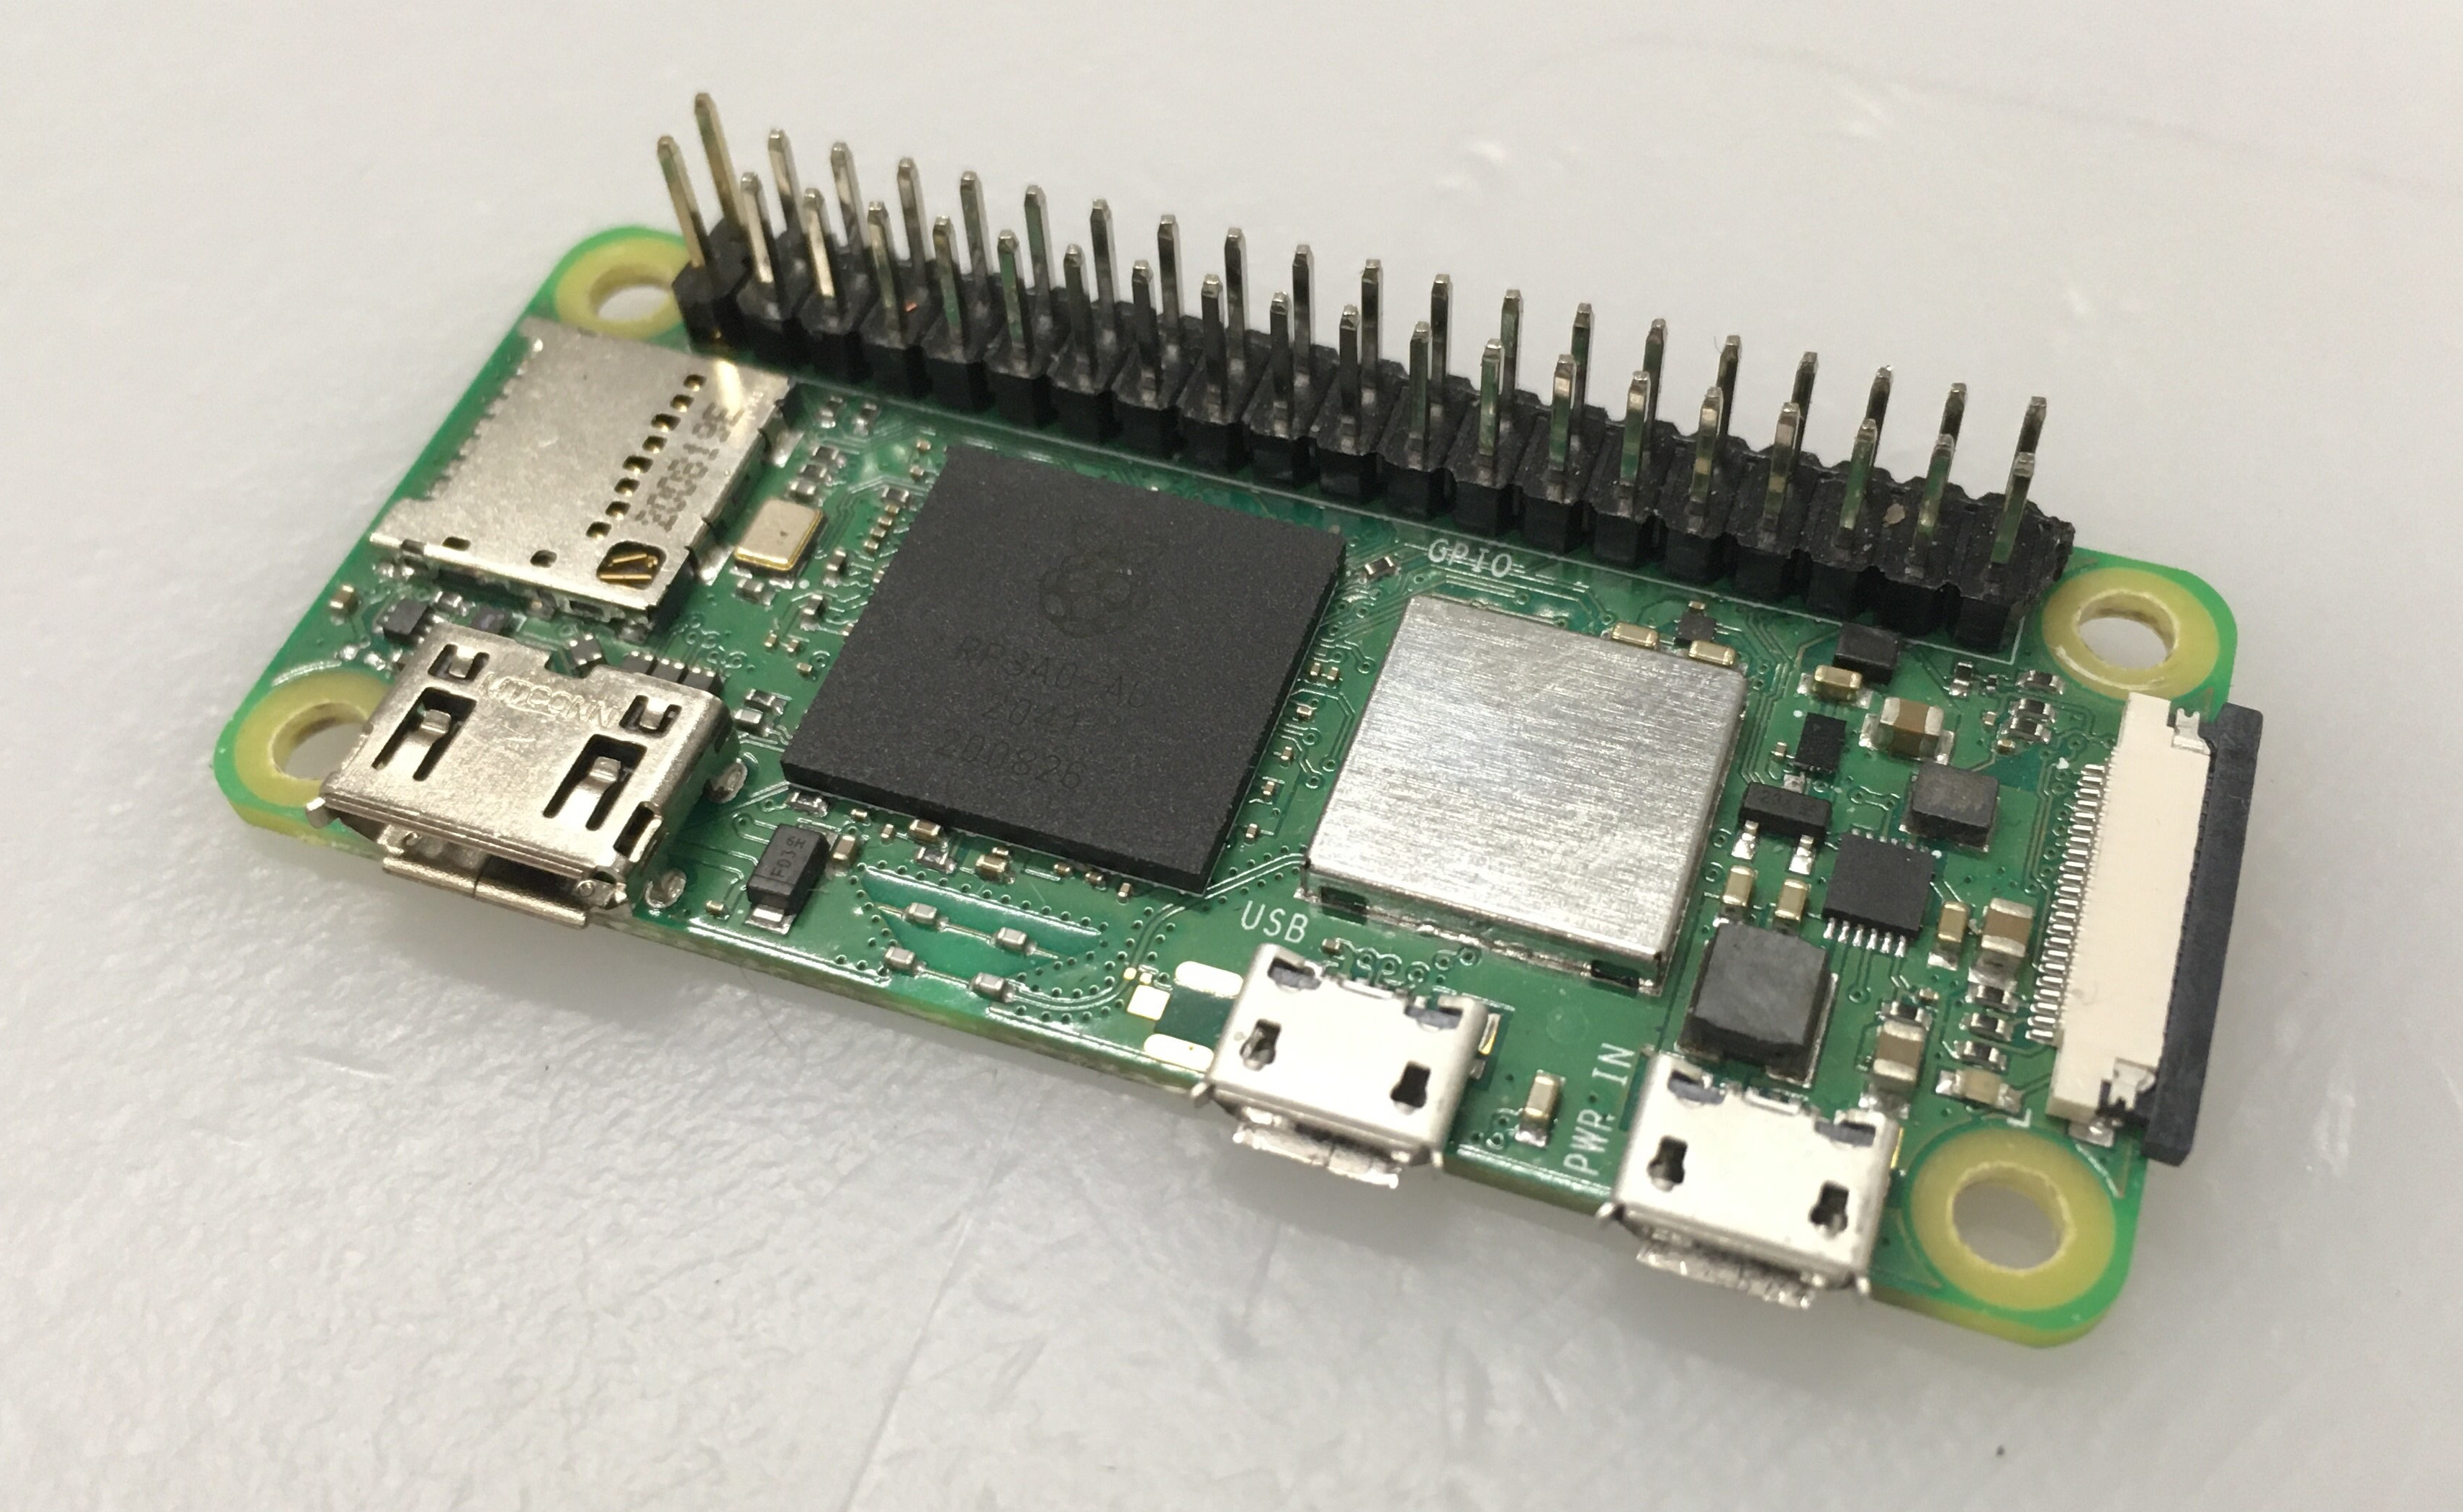
\includegraphics[scale=0.11]{RPi.jpg}
\caption{Raspberry Pi Zero 2 W}
\label{fig:RaspberryPiZero2W}
\end{figure}

\subsection{Raspberry Pi OS}
\label{subsec:tRasPiOS}
Als Betriebssystem für den \ac{Raspi} bietet Raspberry Pi eine auf Debian basierte Linux-Distribution namens Raspberry Pi \ac{OS} an. Raspberry Pi \ac{OS} ist in drei verschiedenen Varianten verfügbar, diese unterscheiden sich im Funktionsumfang und der Installationsgröße. Aufgrund der limitierten Rechenleistung des \ac{Raspi} Zero 2 W und der fehlenden Notwendigkeit für eine Desktop-Umgebung ist die Lite-Version am besten geeignet. Dadurch, dass eine vollwertige Linux-Distribution am Raspberry Pi läuft, kann der \ac{Raspi} Python Code interpretieren und ausführen. Außerdem inkludiert Raspberry Pi OS viele Werkzeuge, darunter das init-System \glqq systemd\grqq , womit einfach Programme mit dem Start des Betriebssystems gleichzeitig gestartet werden können. Ein anderes Werkzeug, das mitgeliefert wird ist der Paketmanager \glqq apt\grqq\ womit Pakete einfach am \ac{Raspi} installiert, entfernt oder aktualisiert werden können.
\begin{figure}[h]
\centering
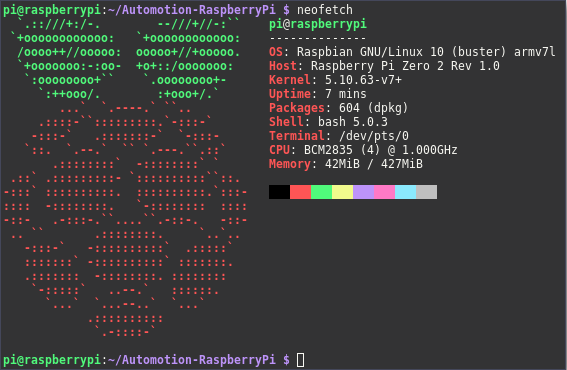
\includegraphics[scale=0.75]{raspineofetch.png}
\caption{Das Commandline-Tool neofetch am Raspberry Pi Zero 2 W}
\label{fig:pineofetch}
\end{figure}

\subsection{Python}
\label{subsec:tPython}
Python ist eine in den frühen 1990ern von Guido van Rossum erstellte Programmiersprache. Heutzutage zeichnet sich Python dadurch aus, dass es quelloffen und für jeden nutzbar ist. Außerdem nimmt Python dem Programmierenden durch die im Vergleich zu Sprachen wie C++ einfache Syntax und das integrierte Ressourcenmanagement viel Arbeit ab. Ein Nachteil von Python ist, dass es im Vergleich mit anderen Sprache wie C++ eine sehr langsame Programmiersprache ist. Aufgrund seiner Simplizität und Verfügbarkeit für Plattformen wie Microsoft Windows, macOS, Linux und FreeBSD gibt es sehr viele quelloffene Bibliotheken für Python, was das Programmieren noch weiter erleichtert. Ein weiterer Unterschied zu Sprachen wie C, C++ oder Rust besteht darin, dass Python interpretiert statt kompiliert wird. Dies hat zur Folge, dass der Code direkt ausgeführt werden kann, solange ein geeigneter Python-Interpreter und die verwendeten Bibliotheken auf dem Zielsystem installiert sind, ohne zuvor für jede Plattform eigens kompiliert werden zu müssen. Der Python Interpreter kann unter Raspberry Pi OS mit dem Befehl \verb|sudo apt install python| installiert werden. Um ein Python-Programm auszuführen, kann der Befehl \verb|python [Dateiname]| verwendet werden.
(\cite{matthes-2019})

\subsection{Python Bibliotheken}
\label{subsec:tLibPython}
Eine Python Bibliothek ist eine Sammlung von verwandten Modulen, sie beinhaltet bestimmte Codestücke, die wiederum in anderen Programmen verwendet werden können. Bibliotheken machen das Programmieren für den Programmierer einfacher und beschleunigen den Prozess des Programmierens. Wenn eine Funktion bereits von jemandem programmiert wurde, muss sie in diesem Fall nicht erneut programmiert werden. Außerdem verkleinern Bibliotheken die Größe des fertigen Programmes, da eine Bibliothek nur einmal auf einem System installiert werden muss und anschließend von mehreren Programmen auf diesem System verwendet werden kann. Oft sind für bestimmte Sensoren Bibliotheken verfügbar, wodurch das Auslesen des Sensors vereinfacht wird. Ein für das Bibliotheksmanagement oft verwendetes Werkzeug ist der Paketmanager \glqq pip\grqq\ , welcher die Aufgabe hat, das Verwalten von Python-Bibliotheken zu vereinfachen. pip kann unter Raspberry Pi OS mit dem Befehl \verb|sudo apt install pip| installiert werden.

\subsubsection{Python Bibliothek: os}
\label{subsubsec:tLibOs}
Diese Bibliothek - dokumentiert auf \url{https://docs.python.org/3/library/os.html} - stellt verschiedene Funktionen bereit, mit welchen mit dem Betriebssystem, auf dem das Programm ausgeführt wird, interagiert werden kann. Unter anderem werden die Funktionen des lesen beziehungsweise schreiben von Dateien oder das interagieren mit Pfaden für den Programmierer vereinfacht. Alle Funktionen dieser Bibliothek funktionieren unter allen von Python unterstützten Betriebssystemen.
(\cite{PythonDocs})

\subsubsection{Python Bibliothek: time}
\label{subsubsec:tLibTime}
Die Bibliothek \glqq time\grqq\ \url{https://docs.python.org/3/library/time.html} bietet eine Vielzahl an Funktionen, welche für zeit-spezifische Python-Programme hilfreich sind. Eine der Funktionen dieser Bibliothek ist das Ausgeben der aktuellen Zeit in Unix-Sekunden beim Aufruf der Funktion \verb|time.time()|. Eine Beispielausgabe dieser Funktion ist \glqq 1648627393.63594\grqq , was umgerechnet \verb|2022-03-30T08:03:13| bedeutet. Andere Funktionen dieser Bibliothek sind die Ausgabe, ob es sich zum Zeitpunkt des Funktionsaufrufes um Tag oder Nacht handelt (abhängig von Sonnenaufgang und Sonnenuntergang), die Ausgabe der aktuellen Zeitzone und der Funktion, den Programmablauf für eine gewisse Zeit zu pausieren.
(\cite{PythonDocs})

\subsubsection{Python Bibliothek: datetime}
\label{subsubsec:tLibDatetime}
Das Modul \glqq datetime\grqq\ (\url{https://docs.python.org/3/library/datetime.html}) stellt Klassen zum Manipulieren von Daten und Zeiten bereit. Dazu zählen Optionen zum Konvertieren von Zeiten zwischen verschiedenen Zeitzonen und das Umwandeln von Zeiten aus Zeichenketten in ein Zeitformat, welches von Bibliotheken wie dem in Sektion \ref{subsubsec:tPyQtGraph} beschriebenen PyQtGraph verwendet werden kann, um die Werte auf die x-Achse auftragen und bei Vergrößerung oder Verschiebung der Ansicht skalieren zu können. Eine weitere Funktion dieser Bibliothek ist das extrahieren von einzelnen Werten aus einem Zeitpunkt, der als ein solcher abgespeichert wurde. Ein Beispiel dafür ist es, das Monat \glqq März\grqq\ aus dem Datum \verb|2022-03-26T17:29:10+01:00| zu entnehmen.
(\cite{PythonDocs})

\subsubsection{Python Bibliothek: shutil}
\label{subsubsec:tShutil}
Die Bibliothek \glqq shutil\grqq\ - dokumentiert unter \url{https://docs.python.org/3/library/shutil.html} - ermöglicht das interagieren mit Dateien, beispielsweise können mithilfe dieser Bibliothek mehrere Dateien gleichzeitig kopiert oder auch entfernt werden. Für das Kopieren von Dateien werden mehrere verschiedene Optionen angeboten, diese unterscheiden sich hauptsächlich daran, dass bei einigen die Metadaten wie zum Beispiel das Erstell- und Bearbeitungsdatum ebenfalls kopiert werden.
(\cite{PythonDocs})

\subsubsection{Python Bibliothek: NumPy}
\label{subsubsec:tNumpy}
NumPy (\url{https://numpy.org/}) ist eine Python Bibliothek, welche viele wissenschaftliche Funktionen wie beispielsweise das Bearbeiten von Arrays, Matrizen und Vektoren vereinfacht. Unter anderem können mithilfe von NumPy die Inhalte von ganzen Arrays mit einer Funktion in einen anderen Datentyp umgewandelt werden. Außerdem kann NumPy einzelne Spalten oder Zeilen aus Arrays ausschneiden und in andere einfügen. Weitere Funktionen von NumPy sind ein eingebauter Zufallszahlengenerator, Fouriertransformationen und das Berechnen von linearer Algebra. NumPy ist teilweise in Python und teilweise in C geschrieben. Alle Funktionen die zeitkritisch sind sind in C implementiert, während Funktionen, bei welchen die Zeit keine Rolle spielt in Python geschrieben sind.
(\cite{NumPyDocs})

\subsubsection{Python Bibliothek: imusensor}
\label{subsubsec:tLibImusensor}
Die Python Bibliothek \glqq imusensor\grqq\ (\url{https://github.com/niru-5/imusensor/tree/master}) stellt verschiedene Möglichkeiten zur Kommunikation zwischen Raspberry Pi und MPU9250 bereit. Einerseits werden Funktionen zur Kalibrierung des MPU9250 angeboten, andererseits werden Funktionen zur Auslesung und Fusion der Messwerte bereitgestellt. Für die Sensorfusion bietet diese Bibliothek zwei verschiedene Filter an, Kalman und Madgwick. Während Kalman simpel ist und nicht sehr viele Prozessorressourcen benötigt, stellt Madgwick glattere Werte bereit, benötigt dafür aber mehr Rechenaufwand.

\subsubsection{Python Bibliothek: pynmea2}
\label{subsubsec:tpynmea2}
pynmea2, verfügbar unter \url{https://github.com/Knio/pynmea2}, ist eine Bibliothek, die zur Interaktion mit dem \ac{NMEA}-Protokoll dient. Die einzelnen \ac{NMEA}-Zeilen, die mit den \ac{NMEA}-Headern beginnen, können geparst werden, somit wird aus den in Abbildung \ref{fig:NMEA} abgebildeten Daten ein lesbares Format generiert, welches anschließend im Programm weiterverwendet werden kann.

\subsubsection{Python Bibliothek: PyQtGraph}
\label{subsubsec:tPyQtGraph}
PyQtGraph (https://www.pyqtgraph.org/) ist eine auf Qt und NumPy basierende Python Bibliothek. Aufgrund ihrer Basis ist diese Bibliothek mit Qt kompatibel und kann mit in bestehende Qt-Anwendungen integriert werden. PyQtGraph stellt viele Funktionen bereit, darunter sowohl das \ac{2D}-Plotten als auch das Zeichnen von \ac{3D} Grafiken mithilfe von OpenGL. Zu den \ac{2D}-Funktionen von PyQtGraph zählen unter anderem Linien- und Streudiagramme mit Skalierungs- und Verschiebungsmöglichkeiten und das Zeichnen von Echtzeitdaten. Zu den \ac{3D}-Funktionen zählen das Rendern von Volumenkörpern, Oberflächen- und \ac{3D}-Streuplots und die Möglichkeit diese zu rotieren oder zu skalieren. Während PyQtGraph in Python geschrieben ist, ist die Bibliothek trotzdem hochperformant, da für die benötigten Berechnungen NumPy verwendet wird, welches wie in \ref{subsubsec:tNumpy} beschrieben C-Code verwendet, um zeitkritische Berechnungen durchzuführen.
(\cite{PyQtGraphDocs})

\subsubsection{Python Bibliothek: py-staticmaps}
\label{subsubsec:tStaticmaps}
Die Bibliothek \glqq staticmaps\grqq\ (\url{https://github.com/flopp/py-staticmaps}) ist sowohl als Python Bibliothek (py-staticmaps) als auch als Go Bibliothek (go-staticmaps) verfügbar. Die Hauptfunktion dieser Bibliothek ist es, das Erstellen von Kartenausschnitten mit diversen Markern und Linien zu ermöglichen. Dazu kann staticmaps automatisch das Zentrum der gegebenen Punkte und die geeignete Zoomstufe berechnen. Außerdem werden verschiedene Anbieter für das Kartenmaterial, darunter \ac{OSM} und ArcGISWorldImagery zur Verfügung gestellt. Die geladenen Kartenabschnitte werden außerdem auf dem Computer, auf dem der Download stattfindet zwischengespeichert, wodurch das erneute Zeichnen der Karte beschleunigt wird. 

\subsubsection{Python Bibliothek: Qt}
\label{subsubsec:tQt}
Qt ist eine von der Qt Company entwickelte Bibliothek für die Entwicklung von grafischen Oberflächen. Sie ist wie Python plattformübergreifend und unterstützt unter anderem Microsoft Windows, macOS, Unixartige Betriebssysteme mit X11, Linux mit Wayland, Android und iOS. Qt unterstützt ebenfalls die Entwicklung mit verschiedenen Programmiersprachen, darunter Python, C++ und Qt Modeling Language, zusätzlich wird Unterstützung für Rust und Go von der Qt-Community angeboten. Qt ist wie Python Quelloffen und kann für die Open-Source-Programmierung frei verwendet werden. Die neueste Qt-Python Bibliothek heißt PySide6, mit nur fünf Zeilen Python-Code kann ein leeres Fenster erstellt werden. Qt stellt außerdem einen Designer bereit, mit welchem grafische Oberflächen in einer grafischen Oberfläche erstellt werden können. Im Qt Designer werden Elemente per Drag and Drop platziert, standardmäßig werden die gängigsten Funktionen einer Desktopanwendung mit \ac{GUI} unterstützt. Es können aber auch Erweiterungen wie zum Beispiel die in Sektion \ref{subsubsec:tPyQtGraph} beschriebene Bibliothek PyQtGraph mithilfe von Qt Designer eingebunden werden.
(\cite{QtDocs})
\begin{figure}[h]
\centering
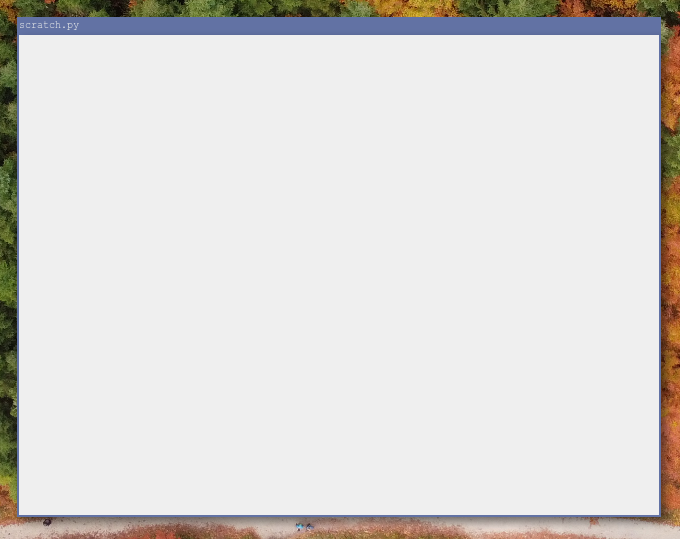
\includegraphics[scale=0.5]{EmptyQtWindow.png}
\caption{Leeres PySide6-Fenster auf Linux unter X11}
\label{fig:EmptyQtWindow}
\end{figure}

\subsection{FDM-3D-Druck}
\label{subsec:tFDM}
\ac{FDM} z. Dt. Schmelzschichtung, ist eine gängige Methode der additiven Fertigung, die auch die Funktionsweise der meisten \ac{3D}-Drucker darstellt. Additive Fertigung bedeutet, dass ein zu herstellendes \ac{3D}-Modell in einzelnen Schichten mit der gewünschten Schichthöhe auf einer Plattform aufgetragen wird. Der Vorteil ist, dass komplexe Modelle gefertigt werden können, die mit herkömmlichen Fertigungsverfahren sehr schwer, oder gar unmöglich produzierbar sind.\\
Bei der \ac{FDM}-Technologie wird ein Kunststoffdraht (Filament) durch eine erhitzte Düse gepresst, wodurch der Kunststoff geschmolzen und je nach Düsenöffnung, in einem bestimmten Durchmesser extrudiert wird. Bei der \ac{FDM}-Methode können also ausschließlich Thermoplaste als Druckmaterial verwendet werden. Die Düse wird während dem Extrudiervorgang in einer bestimmten Höhe über einer (meist beheizten) Plattform, dem sogenannten Druckbett, bewegt, um die erste Schicht des Modells aufzutragen. Anschließend wird die Düse eine Schichthöhe angehoben, um die nächste Schicht auf der ersten aufzutragen (Siehe Abbildung \ref{fig:FDM}). Typische Schichthöhen von \ac{FDM}-Druckern sind 0,1 bis 0,4 Millimeter, die Düse hat meist einen Durchmesser von 0,4 Millimeter. Zu den möglichen Materialien zählen unter anderem \ac{PLA}, \ac{ABS}, \ac{PETG} sowie Nylon. Auch flexible Materialien sind einsetzbar, diese sind allerdings meistens mit erhöhten Druckeranforderungen verbunden. Bei Hobby-Druckern beträgt die typische maximale Druckgröße zwischen 120$\cdot$120$\cdot$120 und 300$\cdot$300$\cdot$300 Millimeter in x-, y-, und z-Richtung. Der große Nachteil von \ac{FDM} ist die Oberflächenbeschaffenheit des fertigen Bauteils, welche markante Rillen der einzelnen Schichten aufweist. (\cite{alexandreFDM})
\begin{figure}[h]
\centering
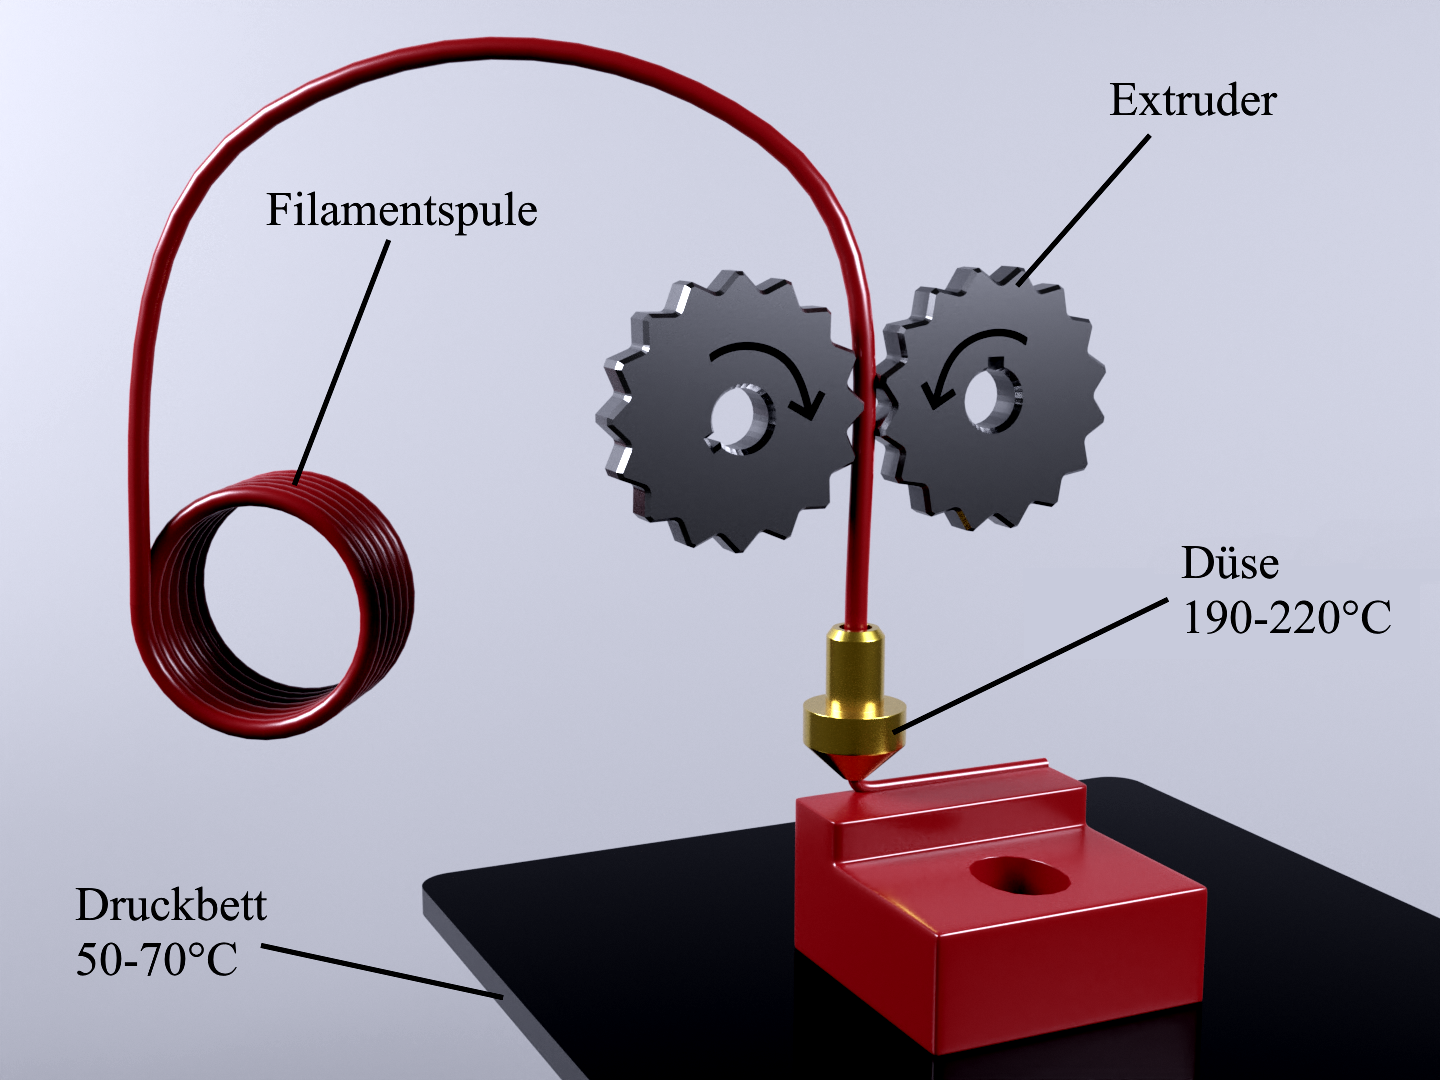
\includegraphics[scale=0.2]{FDM.png}
\caption{FDM-Funktionsweise}
\label{fig:FDM}
\end{figure}

\subsection{DUP-3D-Druck}
\label{subsec:tDUP}
\ac{DUP} ist eines der additiven Fertigungsverfahren, bei dem ein fotosensitives Harz Schicht für Schicht ausgehärtet wird, um ein \ac{3D}-Modell zu fertigen. Bei \ac{DUP} wird eine Plattform kopfüber in einen, mit einem speziellen Harz befüllten, Behälter gesenkt, bis diese eine Schichthöhe vom Boden des Behälters entfernt ist. Der Boden dieses Beckens besteht aus einem durchsichtigen Kunststoff und darunter befindet sich ein \ac{LCD}, welches, anders als herkömmlich, eine \ac{UV}-Leuchtdioden-Matrix als Hintergrundbeleuchtung aufweist. Das \ac{LCD} dient als Schablone und lässt nur dort \ac{UV}-Licht durchscheinen, wo das \ac{UV}-sensitive Harz ausgehärtet (polymerisiert) werden soll. Die erste ausgehärtete Harz-Schicht haftet an der Druckplattform, welche anschließend für die Nächste eine Schichthöhe angehoben wird. Somit wird jeweils eine Schicht auf einmal gefertigt (Siehe Abbildung \ref{fig:DUP}).\\ Harz-Drucker sind bekannt dafür, dass sie eine deutlich bessere Druckqualität liefern können, als \ac{FDM}-Drucker. Der Grund dafür sind zum einen die typischen Schichthöhen von 0.025 bis 0.1 Millimeter sowie die erhöhte Auflösung in x- und y-Richtung, welche abhängig von der \ac{LCD}-Auflösung ist.  Harz-Drucker haben also den großen Vorteil, dass (fast) keine Schicht-Rillen zu erkennen und viel detailliertere Modelle druckbar sind. Die maximale Druckgröße ist in den meisten Fällen kleiner als bei \ac{FDM}-Druckern und liegt im Durchschnitt bei etwa 180$\cdot$120$\cdot$200 Millimeter. Die Wellenlänge des \ac{UV}-Lichts der LEDs beträgt zwischen 395 und 405 Nanometer, diese muss dem sensitiven Bereich des Harzes entsprechen. Nachdem ein Druck fertiggestellt wurde, ist dieses Modell immer noch mit flüssigem Harz überzogen, welches mit Alkohol entfernt werden muss. Da die Aushärtezeit beim Druckprozess pro Schicht nur circa zwei Sekunden dauert, muss das fertige Modell mit einer \ac{UV}-Lichtquelle erneut für 5 bis 10 Minuten ausgehärtet werden, um seine endgültigen Materialeigenschaften zu erhalten. Mittlerweile gibt es einige Unternehmen, welche Harze mit besonderen Eigenschaften anbieten, wie zum Beispiel erhöhte Festigkeit, Zähigkeit oder mechanische Bearbeitbarkeit.\\
\ac{DUP} und andere Harz-Druckverfahren haben also den großen Nachteil, dass sehr viel Aufwand im Bezug auf die Nachbearbeitung besteht und immer mit ausreichend Schutzkleidung, wie Handschuhe und Schutzbrille gearbeitet werden muss, da die Harze gesundheitsschädlich sein können. (\cite{druckwegeDUP})
\begin{figure}[h]
\centering
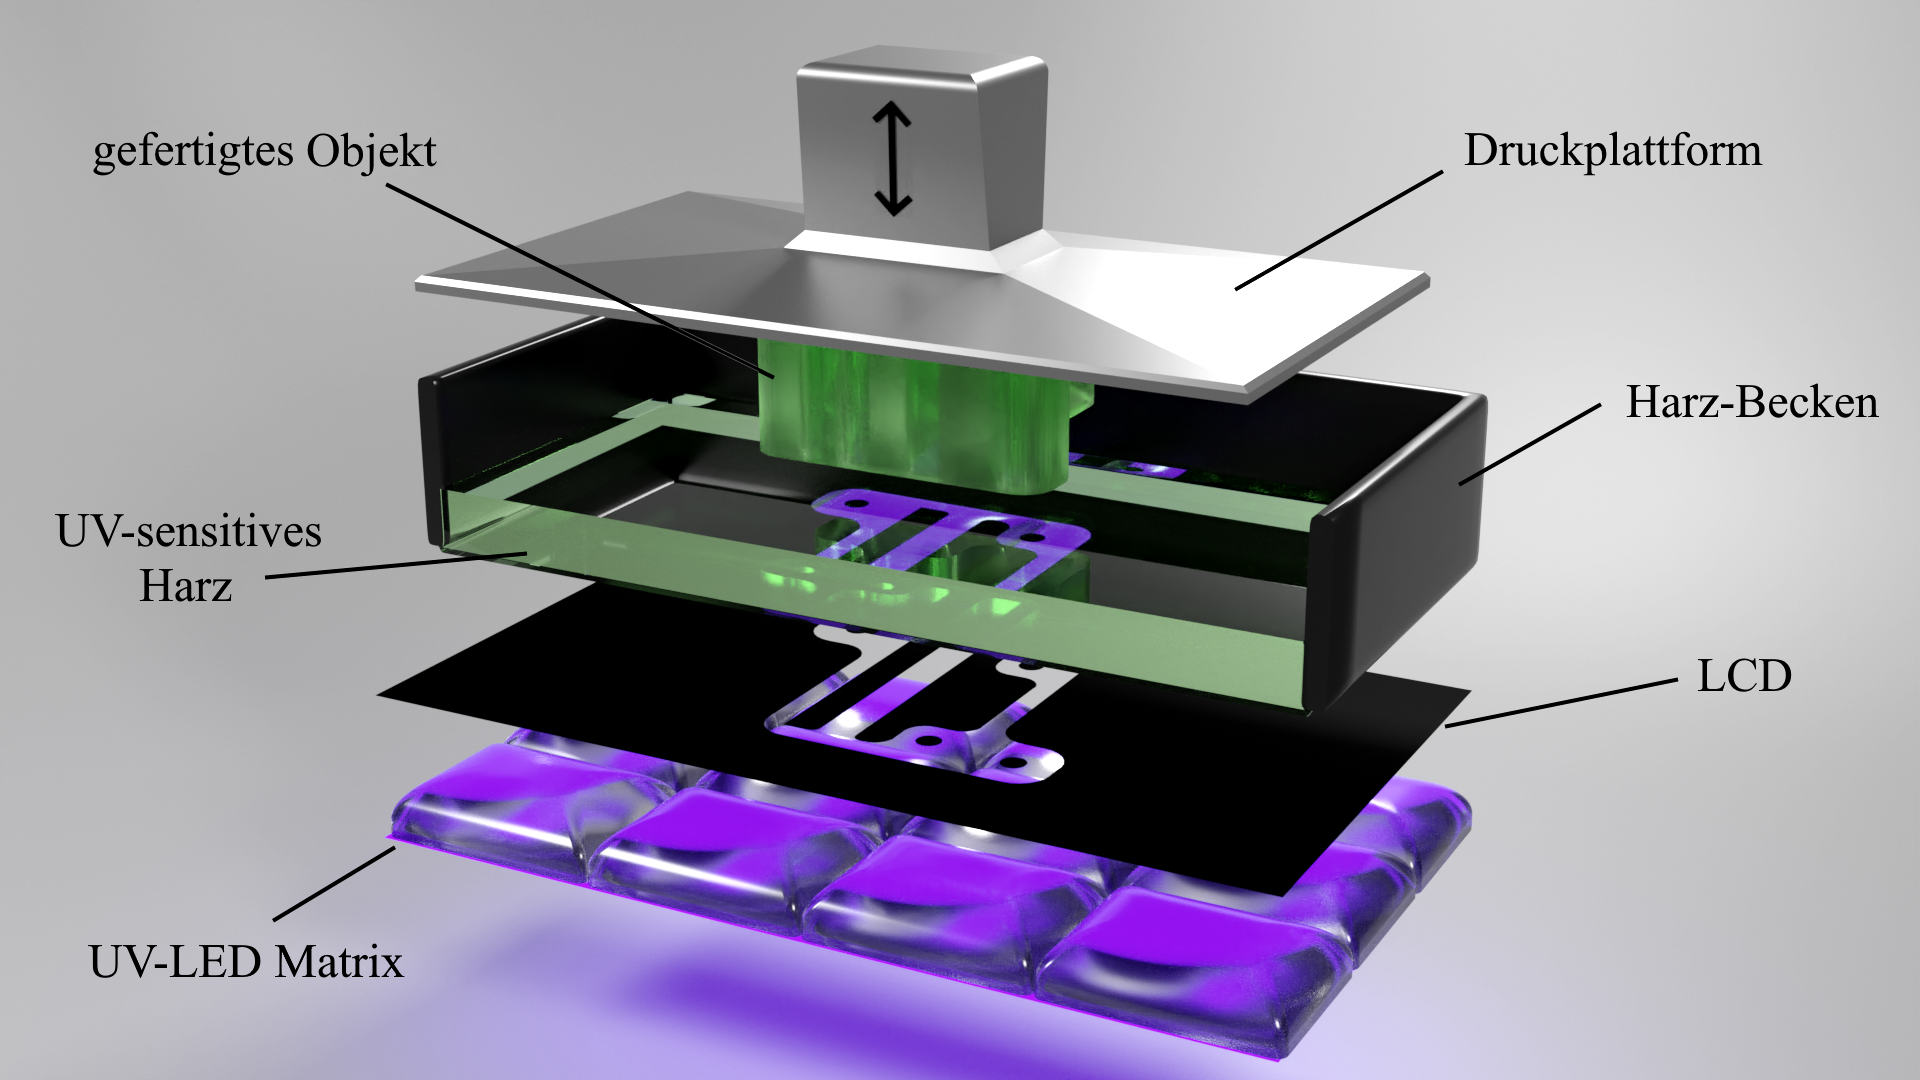
\includegraphics[scale=0.2]{DUP.png}
\caption{DUP-Funktionsweise}
\label{fig:DUP}
\end{figure}

\subsection{Git}
\label{subsec:tGit}
Git ist eine freie und Quelloffene Software, die von Linux Torvalds ins Leben gerufen wurde. Sie unterstützt unter anderem das Verzweigen und Zusammenführen von Code, die Versionsverwaltung des Codes und das kooperative Programmieren. Git kann das gesamte Repository herunterladen, dies geschieht mit \verb|git clone https://github.com/Benibla124/Automotion-Diplomarbeit|. \\ (Dieser Befehl lädt die Quelldateien dieser Diplomarbeit herunter) Mit \verb|git add [Dateiname]| kann eine Datei der Versionsverwaltung hinzugefügt werden, mit \verb|git commit -m "[Nachricht]"|, werden die Änderungen committet, mit \verb|git push| werden die committeten Änderungen hochgeladen. Aufgrund seiner freien und einfachen Nutzbarkeit, wird Git von vielen Firmen, darunter Google, Microsoft, Twitter, Netflix und Facebook verwendet. Wird GIt zur Versionsverwaltung verwendet, können Änderungen jederzeit rückgängig gemacht werden, da Git jede Version für immer abspeichert. Git ist unter anderem für Linux, FreeBSD, macOS, Solaris und Microsoft Windows verfügbar.
(\cite{GitDocs})